\chapter{Cooling}
\label{chap:Cooling}
A prerequisite for performing photon recoil spectroscopy, is that the system which is investigated, is cooled to the quantum mechanical ground state of its motion.
Cooling of ions in linear Paul traps usually occurs in two stages. First the ion(s) is cooled to approx. 0.5mK by Doppler cooling, as is described in \cref{sec:Doppler}.

When the ion(s) has been cooled to mK temperature by Doppler cooling, it starts exhibiting quantum mechanical properties. Since the potential in the trap is harmonic, the wave function of the ion(s), is that of the harmonic oscillator.
To reach the quantum ground state, it is necessary to perform sideband cooling which takes the ion(s) from whichever distribution over the Fock states $\vert n\rangle$ it starts in, and moves it to the ground state $\vert0\rangle$. This process is described in \cref{sec:SBC}.

Complications arise in the above cooling processes, if we consider two ions with very large charge-to-mass mismatch. A potential solution to the issues that arise is given in \cref{sec:Coupling}.
\section{Doppler cooling}
\label{sec:Doppler}
The very first part of cooling ions consists of Doppler cooling \cite{WinelandLaserCool}. This method of laser cooling was pioneered by David Wineland and relies on detuning laser light with respect to an internal transition of the ion, in order to effectively generate a drag force on the ion, cooling it down.

An ion travelling at some a velocity $\vec{v}$, experiences a Doppler shift of laser light with wave vector $\vec{k}$ according to
\begin{equation}
    \omega_{obs} \approx (1-\vec{k}\cdot\vec{v})\omega_L,
\end{equation}
where $\omega_{obs}$ is the frequency seen by the ion, and $\omega_L$ is the frequency of the laser in the laboratory frame.
Thus, if we detune the light of the laser to be below the frequency $\omega$ of an electronic transition in the ion, the ion will preferentially absorb photons, when it is propagating against the direction of the light.
Due to conservation of momentum, the momentum of the ion must change whenever absorption occurs, this change is given as
\begin{equation}
    \Delta\vec{p} = \hbar\vec{k}.
\end{equation}
Shortly after absorption, the ion will decay to the ground state once again. Naturally, this process changes the momentum of the ion once more. Since the direction photons are emitted in under spontaneous decay is symmetric, the change in momentum due to spontaneous emission will average out over the course of several emissions.


Thus, the momentum of the ion is effectively decreased, since the ion preferentially absorbs photons propagating in the opposite direction of itself, each time changing its momentum by $\hbar\vec{k}$. At low velocities $kv\ll\Gamma$, where $\Gamma$ is the decay rate of the excited state, one can express this as a drag force (assuming 1D problem to ease notation) \cite{Fisher_2017}:
\begin{equation}
    F_{drag} = -\beta v,\quad \beta = \frac{8\hbar s k^2\delta / 2\Gamma}{\big(1+s+(2\delta/\Gamma)^2\big)^2},
\end{equation}
where $\beta$ is the drag coefficient, $\delta = \omega_L-\omega$ is the detuning of the laser with respect to the atomic transition, $s = I/I_{sat}$ is the saturation parameter, which is calculated from the intensity of the laser light $I$, and the saturation intensity $I_{sat} = \frac{\pi hc}{3\lambda}\Gamma$, with $\lambda$ being the wavelength of the laser. 

It is important to note, that while the equation above seems to indicate that there is no limit to Doppler cooling, that is not the case. Indeed, since the direction of an emitted photon is random, the ion will perform a random walk in momentum space over time.
Thus, there is an intrinsic variation of velocity over time, resulting in a lower limit to the temperature of the ion (typically referred to as the Doppler temperature or Doppler limit), which is given by
\begin{equation}
    T_D = \frac{\hbar\Gamma}{2k_b}\label{eq:DopplerTemp}.
\end{equation}
For Doppler cooling on the $\text{S}_{1/2} \rightarrow \text{P}_{1/2}$ transition of Ba$^+$, which has a linewidth of $2\pi\times 15.2$MHz, this results in a Doppler temperature of approx. 0.5mK.

Of course, Doppler cooling only works for very specific ions, that have the proper level-scheme, and is thus not a very good candidate for cooling arbitrary molecular ions.
The solution to this problem, is to trap ions that \textit{can} be cooled alongside the molecule. Since both the atom(s) and the molecule carry charge they will interact via the Coulomb interaction. Such interactions will cause the molecular ion to transfer energy to the atomic ion, from which the energy will then be removed from the system via Doppler cooling. This method of cooling is called sympathetic cooling \cite{StefanSympa,MichaelSympa}.

As temperatures drop low enough that the motion becomes harmonic, the motion of the atomic and molecular ion becomes coupled. As such, the ions will have common motional modes, and any energy extracted from the Ba$^+$ ion is extracted from the mode as a whole, thus cooling the molecular ion as well.
This cooling mechanism is only effective if the ions share similar mass-to-charge ratios, however. In the case where the ion motions are nigh uncoupled, as described in \cref{sec:2Ion}, further steps must be taken to get the molecular ion to mK temperatures. This is described in \cref{sec:Coupling}.


\section{Sideband Cooling}
\label{sec:SBC}
Unfortunately, Doppler cooling is not sufficient for reaching the motional ground state. To do this, we employ yet another method of laser cooling, called sideband cooling \cite{WinelandSideband}. When the ions are at the Doppler temperature, they will be cold enough that they behave as a quantum mechanical harmonic oscillator, with their wave function
being a thermal distribution over the Fock states $\vert n \rangle$. By coupling the state $\vert g,n\rangle$ to the state $\vert e,n-1\rangle$, where $(e,g)$ denotes the excited and ground states of the atom, we are able to remove one quantum of energy from the motion under an excitation of the electronic state.
Since the state $\vert e,n\rangle$ predominantly decays to the state  $\vert g,n\rangle$, this allows us to cool the ion's motion by moving down the "ladder" seen on \cref{fig:SBC}


To understand sideband cooling from a theoretical point of view, we initially consider a one-ion system, and ignore the radial motion to ease notation. The Hamiltonian can be written as
\begin{equation}
    \hat{H}_0 = \hbar\omega_{z}(\hat{n}+1/2)+\hat{H}_a,
\end{equation}
where $\hat{n}$ is the Fock state number operator, and $\hat{H}_a$ is the Hamiltonian for the atomic system. If a laser field is turned on at some detuning $\delta = \omega_L -\omega$ with respect to the electronic transition of the ion, the interaction with the laser can be written in the interaction picture as:
\begin{equation}
    H_{I} = \frac{\hbar\Omega_0}{2}\hat{\sigma}_+\big(e^{ik_z\hat{z_I}}e^{-i\delta t}\big) + h.c.,
    \label{eq:interaction}
\end{equation}
where $\hat{\sigma}_+ = \vert e \rangle \langle g \vert$ is the excitation operator responsible for exciting the electronic state of the ion, and $\Omega_0 = \frac{eE_0}{\hbar}\langle g \vert \hat{\epsilon}\cdot\hat{z}\vert e\rangle$ is the Rabi frequency of the transition, being driven by an electric field of amplitude $E_0$, and direction $\hat{\epsilon}$. Note that the rotating wave approximation has been applied to the expression above, keeping only slowly rotating terms.

We may express $\hat{z}_I$ in terms of the ladder operators yielding
\begin{equation}
    \hat{z}_I = \sqrt{\frac{\hbar}{2m\omega_z}}(\hat{a}e^{-i\omega_z t}+\hat{a}^\dagger e^{i\omega_z t}).
\end{equation}
Before inserting this expression back into \cref{eq:interaction}, it will be useful to first define the Lamb-Dicke parameter
\begin{equation}
    \eta = k_z\sqrt{\frac{\hbar}{2m\omega_z}},
\end{equation}
which in the so-called Lamb-Dicke regime, where $\eta\sqrt{\langle n \rangle +1} \ll 1$ \cite{PRS} allows us to write
\begin{equation}
    H_I = \frac{\hbar\Omega_0}{2}\hat{\sigma}_+\bigg[e^{-i\delta t} + i\eta\big(\hat{a}^\dagger e^{i(\omega_z -\delta)t}+\hat{a}e^{-i(\omega_z+\delta)t}\big)\bigg] + h.c.
    \label{eq:interactionPic}
\end{equation}
Here the first term is resonant when $\delta = 0$ and corresponds to the laser being resonant with the atomic transition, driving it with no change in motional quantum number. The second term is resonant when the laser is blue detuned by  $\delta = \omega_z$, and increases the motional quantum number while exciting the system, thus heating the system, corresponding to walking up the ladder of \cref{fig:SBC}.
Finally, the third term is resonant when $\delta = -\omega_z$, and excites the atomic ion, at the cost of a phonon. Since the atom will predominantly decay to the same $\vert n\rangle$ state, repeating this process will eventually cool the ion to the ground state, as seen on \cref{fig:SBC}.

If we instead consider two ions, the picture changes ever so slightly. In the case where only one of the ions interacts with the laser light, as would be the case for Ba$^+$ cotrapped with a molecule, we must include the mode structure when writing out the position operator. In the case of two ions with in-phase and out-of-phase frequencies $\omega_i,\omega_o$, the motional state of the system is described by the product space $\vert n_i,n_o\rangle$,
with the subscript ($i/o$) denoting the in-phase and out-of-phase mode respectively. Including the mode structure, can be done by performing the substitution

\begin{equation}
    \hat{z_I}\rightarrow\hat{\xi}_{1,I} = \sqrt{\frac{\hbar}{2m_1}}\bigg(\alpha_{i,1}\frac{\hat{a}_ie^{-i\omega_it}+\hat{a}_i^\dagger e^{i\omega_i t}}{\sqrt{\omega_i}}+\alpha_{o,1}\frac{\hat{a}_oe^{-i\omega_o t}+\hat{a}_o^\dagger e^{i\omega_o t}}{\sqrt{\omega_o}}\bigg),
\end{equation}
in \cref{eq:interactionPic}, where $\alpha_{i/o,1}$ is the participation of the atomic ion in the motion of the mode, as calculated in \cref{sec:2Ion}. Following an identical derivation we see that sideband cooling is still possible for all modes, provided that $\alpha_{i/o}$ isn't too small.

This clearly poses a problem for systems where the mass-to-charge ratios of the two ions differ considerably, as $\alpha_{i,1}\ll \frac{1}{\sqrt{2}}$ for such systems. Effectively making cooling of the in-phase (or out-of-phase for the radial case) motion impossible. A potential solution to this problem is presented in \cref{sec:Coupling}.

\begin{figure}
    \centering
    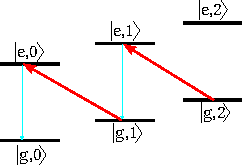
\includegraphics[width = 0.8\textwidth]{main/coolingScheme.pdf}
    \caption{Illustration of the concept behind sideband laser cooling. The laser (red) is detuned with respect to the electronic transition, by exactly $\omega_z$. Thus, transitions are driven at the cost of a phonon. The atom is most likely to decay (blue) to the same Fock state, effectively causing it to lose phonons, over several excitations. This makes the ion "climb down the ladder" until it reaches the quantum ground state}
    \label{fig:SBC}
\end{figure}

\section{Coupling of motional modes to enhance cooling}
\label{sec:Coupling}
As mentioned in both \cref{sec:Doppler} and \cref{sec:SBC}, laser cooling becomes very difficult once the charge-to-mass ratios of the two differ considerably. The reason for this is relatively easy to understand.
Since the laser cooling only interacts with the atomic ion, this is the only ion whose motion is cooled directly through the interaction with the light. In the case where the ions have similar charge-to-mass ratios however, their motions are so strongly coupled, that any cooling of the atomic ion, will cool the molecular ion as well.
As the ratios start to differ, the motions quickly become uncoupled, and thus the cooling of the atom no longer affects the molecule in any appreciative way. This is seen on \cref{fig:WCMSCM}, which shows the temperature of a Ba$^+$ ion, cotrapped with a polyporphyrin ($m_2 = 9000$ amu, $q_2 = 24$e). The blue curve shows the temperature of the motional modes, that have a large contribution from the atom. Clearly these modes are effectively cooled. In stark contrast we have the orange curve, which displays the temperature of all the modes that have low contribution from the atom, whose temperature remains effectively unchanged.

\begin{figure}
    \centering
    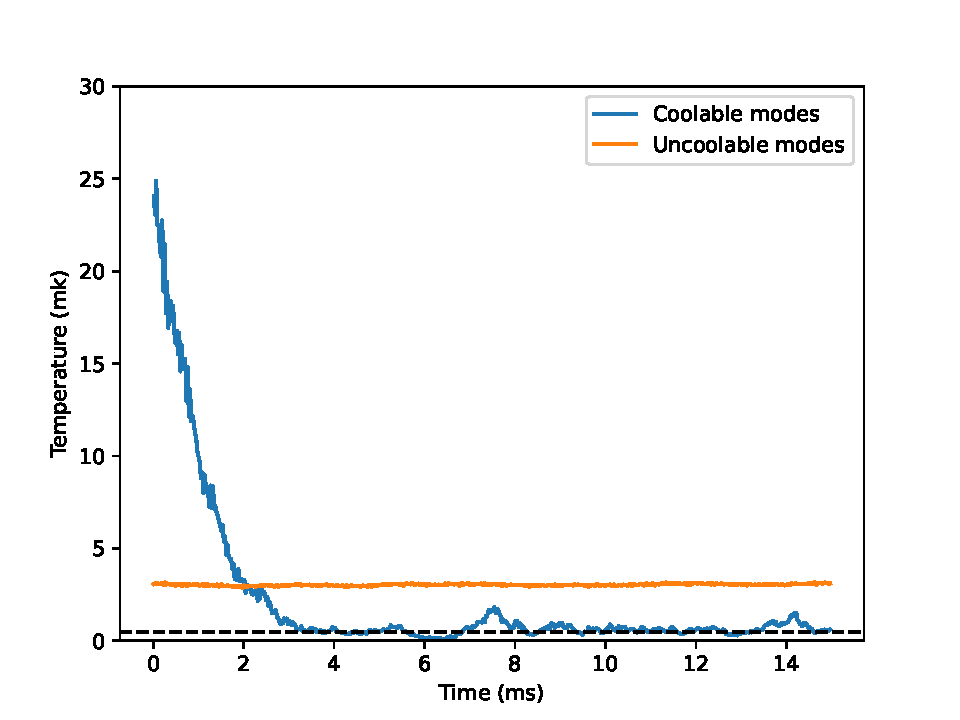
\includegraphics[width = \textwidth]{main/WCM_SCM_Temp.pdf}
    \caption{Simulation of Doppler cooling in all three dimensions of a two-ion system, consisting of a Ba$^+$ ion, and a polyporphyrin. Two curves are plotted, corresponding to the temperature of the modes with high (blue), and low (orange) participation from the Ba$^+$ ion. Only the modes with a high participation appear to be cooled by the Doppler cooling. Temperature has been determined by calculating $\langle v^2\rangle$, averaging over 100 RF cycles}
    \label{fig:WCMSCM}
\end{figure}

In fact, this problem reaches further than simply cooling. For example, it is the molecular ion we wish to investigate with photon recoil spectroscopy (PRS). However, the momentum kick gained from absorption on the molecule, will predominantly excite the motional modes with high participation from the molecule.
Unfortunately, the readout method for PRS is very similar to the side-band pulses described in \cref{sec:SBC}, and thus, readout becomes impossible when the coupling grows too weak, since these modes have very small participation from the atomic ion, on which readout is performed.


The solution to this problem is to find some way to couple the two modes, allowing for the transfer of energy from one to the other. Curiously, the need for coupling such modes was present in Penning traps many years ago, where mode coupling was necessary in order to cool the so-called magnetron mode of such a trap \cite{PenningTrap,DehmeltPenningCool}. For the Penning trap, the solution found was to add another quadrupole field, oscillating at the frequency difference between the two modes to be coupled. Such a solution also works for the case of the Paul trap, as has been demonstrated very recently \cite{WeaklyCoupled}.

To understand why such a field couples the modes, it is most instructive to consider the quantum mechanical case. Suppose we introduce some additional potential (by modulating a slight additional voltage on the endcap electrodes)
\begin{equation}
    V'(z_1,z_2,t) = \frac{\kappa V_0}{z_0^2}(q_1z_1^2+q_2z_2^2)\cos{\big([\omega_i-\omega_o]t\big)}\label{eq:couplingPot},
\end{equation}
where $V_0$ is the additional voltage put onto the endcap electrodes. We note that $V_0$ is kept small with respect to $V_{DC}$, such that the eigenmodes of the system are not considerably changed.

If we perform a Taylor expansion to second order around the equilibrium positions (at $V_0= 0$) similarly to \cref{sec:2Ion}, we may write (neglecting the offset term)
\begin{align}
    V'(\delta z_1,\delta z_2,t)\approx &\frac{1}{\sqrt{m_1}}\frac{\partial V'}{\partial z_1}\bigg\vert_{eq}\xi_1+\frac{1}{\sqrt{m_2}}\frac{\partial V'}{\partial z_2}\bigg\vert_{eq}\xi_2
    \\&+\frac{1}{2 m_2}\frac{\partial^2 V'}{\partial z_1^2}\bigg\vert_{eq}\xi_1^2\nonumber+\frac{1}{2m_2}\frac{\partial^2 V'}{\partial z_2^2}\bigg\vert_{eq}\xi_2^2,
\end{align}
where we've once again transformed into the mass-weighted displacement coordinates of\cref{sec:2Ion}.
For now, we only wish to consider the coupling of the modes, and thus neglect the first-order terms. Clearly these terms cannot couple the modes as $\hat{\xi}_j \propto (\alpha_{j,o}\hat{a}_o+\alpha_{j,i}\hat{a}_i)+h.c.$ is not sufficient to transfer energy from one mode to another. If we instead consider only the 2nd order terms, we find
\begin{align}
    \hat{V}'^{(2)} = \nonumber \frac{\hbar\kappa V_0}{2z_0^2}\cos{\big([\omega_i-\omega_o]t\big)}\bigg(&q_1\big(\frac{\alpha_{1,i}(\hat{a}_i+\hat{a}_i^\dagger)}{\sqrt{m_1\omega_i}}+\frac{\alpha_{1,o}(\hat{a}_o+\hat{a}_o^\dagger)}{\sqrt{m_1\omega_o}}\big)^2\\
    &+q_2\big(\frac{\alpha_{2,i}(\hat{a}_i+\hat{a}_i^\dagger)}{\sqrt{m_2\omega_i}}+\frac{\alpha_{2,o}(\hat{a}_o+\hat{a}_o^\dagger)}{\sqrt{m_2\omega_o}}\big)^2\bigg).
\end{align}
If the cosine is expanded using Euler's formula, and we move to the interaction picture, keeping only the non-rotating terms, we may massage the expression and eventually arrive at
\begin{equation}
    \hat{V}'^{(2)}_I = \frac{\hbar\kappa V_0\alpha_{1,o}\alpha_{1,i}}{4z_0^2\sqrt{\omega_i\omega_o}}\big(\frac{q_1}{m_1}-\frac{q_2}{m_2}\big)(\hat{a}_o^\dagger \hat{a}_i + h.c.),
\end{equation}
for which it is clear that the two modes of motion are coupled. We define $g_0 = \frac{\kappa V_0\alpha_{1,i}\alpha_{1,o}}{4z_0^2\sqrt{\omega_i\omega_o}}(\frac{q_1}{m_1}-\frac{q_2}{m_2})$, that we may write the coupling potential as 
\begin{equation}
    \hat{V}_I'^{(2)} = \hbar g_0(\hat{a}_i^\dagger \hat{a}_o + h.c.).
\end{equation}
It can be shown, that in the coupled system the time-dependent operators $\hat{a}_{i/o}^\dagger(t)$, are given by \cite{hou2022coherently}
\begin{align}
    &\hat{a_i}^\dagger(t) = \hat{a}_i^\dagger(0)\cos(g_0t) + i\hat{a}_o^\dagger\sin(g_0t),\\
    &\hat{a_o}^\dagger(t) = \hat{a}_o^\dagger(0)\cos(g_0t) + i\hat{a}_i^\dagger\sin(g_0t).
\end{align}
For which it is particularly interesting to note that for times $\tau_n = \frac{(2n+1)\pi}{2g_0}$, where $n$ is an integer, we find that $\hat{a}_i^\dagger(\tau_n) = \hat{a}_o^\dagger(0)$, and similarly for $\hat{a}_o^\dagger(\tau_n)$. In addition, we may write any arbitrary state of the system as
\begin{equation}
    \vert \Psi(t)\rangle = \sum_{m,n = 0}^\infty \frac{c_{mn}}{\sqrt{m!n!}}\big(a_i^\dagger(t)\big)^m\big(a_o^\dagger(t)\big)^n\vert 0\rangle_i\vert 0\rangle_o,
\end{equation}
where the time-dependance of the system is fully captured by the creation operators \cite{hou2022coherently}, the values $c_{mn}$ are determined by the initial state of the system, and $\sum \vert c_{mn}\vert^2 =1$.
The action of the coupling is thus clear. In general, the coupling causes the two states to oscillate in and out of entanglement, and specifically for times $t = \tau_n$ the states of the two modes become swapped.
This is very beneficial for cooling, since we may cool the mode with high participation from the Ba$^+$ ion to the ground state, perform a swap, and then cool again. This procedure should lead to both modes being in their ground states.


The mode coupling also exists in the classical regime. \Cref{fig:polyPorCooling} shows a simulation of Doppler cooling of a system consisting of a  Ba$^+$ ion, and a polyporphyrin, while the coupling $V'$ is turned on. Clearly the molecular ion is able to reach the Doppler temperature of 0.5mK indicated by the dark dotted line on the inset. This stands in stark contrast to \cref{fig:WCMSCM}, where the temperature of the molecule is unchanged.
\begin{figure}[h]
    \centering
    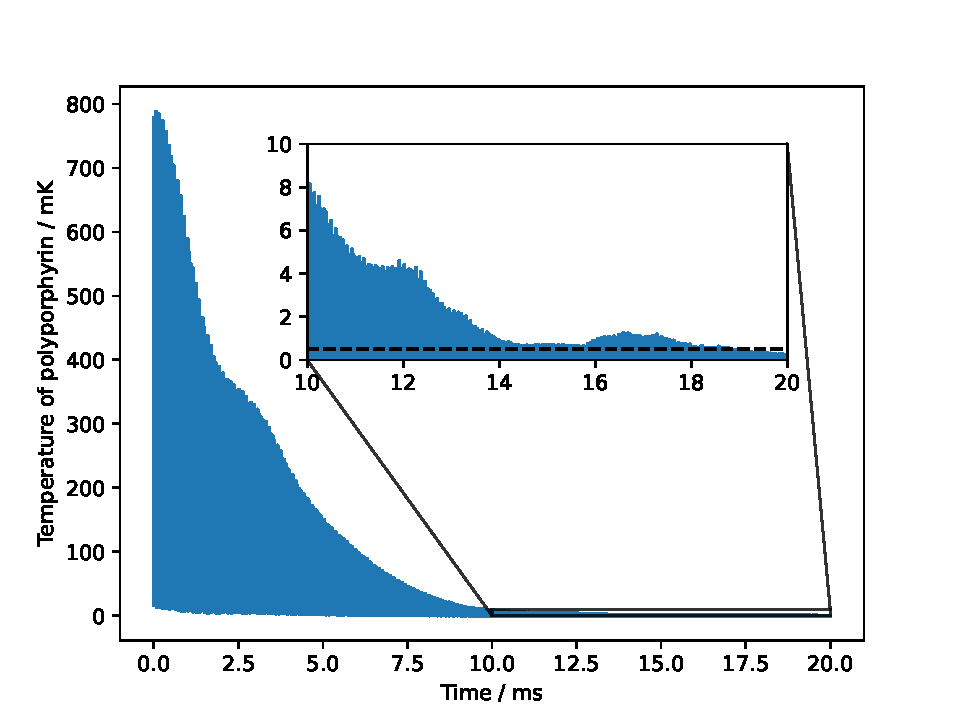
\includegraphics[width = 0.8\textwidth]{main/PolyPorCooling.pdf}
    \caption{Simulation results for the temperature of a polyporphyrin's motion in the $z$-direction. The polyporphyrin is co-trapped with Ba$^+$, which is being Doppler cooled while the coupling potential from \cref{eq:couplingPot} is turned on at a voltage equal to 5\% of the DC voltage. Unlike the case with no coupling (\cref{fig:WCMSCM}), the molecule is cooled efficiently.
    The inset shows temperatures during the interval $t = $10ms to $t = $20ms, as temperatures grow so small that they are not clearly seen on the full figure. The black dotted line shows $T = 0.5$mK, which is the Doppler temperature, calculated by \cref{eq:DopplerTemp}. Once again temperature has been calculated by determining $\langle v^2\rangle$, averaging over 100 RF cycles}
    \label{fig:polyPorCooling}
\end{figure}
\medskip
In the derivations of this section we have ignored the 1st order terms of the Taylor expansion of the potential $V'$. In reality, these terms will play a role in the dynamics of the system, since they drive the ions at a frequency, which is similar to their motional frequencies. There are several ways to combat these first order driving terms.
One option, which has been implemented for the case of segmented microtraps, is engineering the field curvature in order to ensure the first order derivatives go to zero at the equilibrium locations of the ions \cite{WeaklyCoupled}. 

Since our trap has considerably fewer segments than most microtraps, such an approach is expected to be difficult to realize in our setup.
The second approach accepts that the driving terms will lead to heating, but attempts to move this heating into the modes which are easily cooled, i.e. the ones with high participation from Ba$^+$. This can be done by biasing voltages slightly, such that the transfer potential $V'(z_1,z_2,t)$ is zero at $z_{2,eq}$, instead of $z=0$.
We believe this would be relatively simple to implement in the current trap, as a similar thing is already done in order to compensate for micromotion.\\


The usefulness of mode coupling doesn't stop at laser cooling. As mentioned previously, when performing PRS we will largely excite the motion of the molecule. Mode-coupling allows for the efficient mapping of the motion of the molecule onto the motion of the ion making it possible to perform PRS, even with ions that have large mismatches in charge-to-mass ratio.


The contents of \cref{chap:LinTrap} and the current chapter have also been used in the authoring of a paper, proposing an experiment to set bounds on a quantum collapse model, known as the continuous spontaneous localization model \cite{lenlereriksen2023testing}. Using the theory of \cref{sec:2Ion}, we found the strongest bounds on the models parameters could be set by performing measurements on the modes with high participation from the molecular ion, yielding another case where mode-coupling can be highly beneficial.
